\documentclass[11pt,a4paper]{article}

\usepackage[T1]{fontenc}
\usepackage[utf8]{inputenc}
\usepackage[english]{babel}
\usepackage{amsmath,amssymb,mathtools}
\usepackage{geometry}
\usepackage{graphicx}
\usepackage{booktabs}
\usepackage{hyperref}
\usepackage{enumitem}
\usepackage{float}

\geometry{margin=2.5cm}
\hypersetup{
  colorlinks=true,
  hypertexnames=false,
  linkcolor=blue,
  citecolor=blue,
  urlcolor=blue
}
\graphicspath{{outputs/}}

\newcommand{\CCIsoc}{\mathrm{CCI}_{\mathrm{soc}}}
\newcommand{\ASIsoc}{\mathrm{ASI}_{\mathrm{soc}}}
\newcommand{\Seff}{S_{\mathrm{eff}}}
\newcommand{\Rresp}{R_{\mathrm{resp,soc}}}
\newcommand{\Rrob}{R_{\mathrm{rob,soc}}}
\newcommand{\Rsig}{R_{\mathrm{sig,soc}}}

\title{
\textbf{Societal Critical Coherence Index}\\[0.4em]
\large A Toy Framework for Structural Stress and Constructive Transformation
}

\author{
Christof Krieg\\
\small MAAT Project -- Independent Research\\
\small \url{https://maat-research.com}
}

\date{2026}

\begin{document}

\maketitle

\begin{abstract}
We introduce a synthetic and ethically bounded toy framework for applying
the Critical Coherence Index logic to social-system archetypes.
The goal is not to rank real people, parties, countries, organisations, or
communities, but to test whether structural diagnostics can separate raw
activity, passive coherence, robustness, and constructive transformation.

The framework defines four primitive support variables: coherence $H$,
balance $B$, raw social activity $A_{\mathrm{raw}}$, and connectedness $V$.
Raw activity is converted into controlled activity through an optimal-window
response $\Seff(A)$, so that both stagnation and overdriven mobilisation are
penalised.
From these quantities we construct passive structural adherence $\Rresp$,
activity-sensitive robustness $\Rrob$, active societal significance $\Rsig$,
a societal structural-stress index $\CCIsoc$, and a constructive-significance
index $\ASIsoc$.

A reproducible fixed-seed simulation evaluates six synthetic archetypes and a
5000-sample random ensemble.
The highest constructive-significance score is obtained by the
\emph{creative democratic renewal} archetype
($\ASIsoc\simeq0.694$, $\Rsig\simeq0.906$), while the highest structural
stress is obtained by \emph{polarized mobilisation}
($\CCIsoc\simeq1.018$).
The result supports the distinction between low stress, high activity, and
constructive transformation.
\end{abstract}

\section{Purpose and Ethical Status}

This paper is an experiment in structural analogy.
It transfers the MAAT/CCI idea from physical and computational systems to a
synthetic social-system toy model.
It is deliberately not a social scoring system.

\begin{quote}
\emph{Social health is not the absence of conflict, but the capacity to
transform conflict into coherent, balanced, and connected activity.}
\end{quote}

The model must not be used to rank real people, parties, countries,
organisations, populations, or communities.
All examples are synthetic archetypes designed to test regime separation.
The output should be interpreted as a conceptual diagnostic and not as a
normative judgement.

\section{From Physical CCI to Social-System Diagnostics}

The original Critical Coherence Index was introduced as a structural
diagnostic balancing activity and coherence in nonlinear systems.
In the present paper we do not claim a literal physical derivation for social
systems.
Instead, we use the CCI logic as a controlled analogy for complex social
states.

The central hypothesis is:
\begin{quote}
\emph{Activity is not automatically constructive, and stability is not
automatically healthy. Constructive transformation requires controlled
activity constrained by coherence, balance, and connectedness.}
\end{quote}

\section{Societal Support Sectors}

The toy model uses four primitive support variables.
The fifth quantity, robustness or respect, is not treated as an independent
primitive sector.
Instead, it is derived as an emergent closure from the primitive supports,
consistent with the MAAT v1.2.1 convention.

\begin{table}[H]
\centering
\caption{Primitive and derived social-system quantities in the toy model.}
\begin{tabular}{lll}
\toprule
\textbf{Symbol} & \textbf{Role} & \textbf{Social interpretation} \\
\midrule
$H$ & primitive support & coherent orientation, shared sense-making \\
$B$ & primitive support & balance between social tensions \\
$A_{\mathrm{raw}}$ & raw activity & mobilisation, reform pressure, civic activity \\
$V$ & primitive support & trust, communication, connectedness \\
$\Seff$ & derived support & controlled activity in an optimal window \\
$\Rresp$ & derived closure & passive structural adherence \\
$\Rrob$ & derived closure & activity-sensitive robustness \\
$\Rsig$ & derived diagnostic & active constructive significance \\
\bottomrule
\end{tabular}
\end{table}

\section{Controlled Activity}

Raw activity is not treated as intrinsically positive.
Too little activity corresponds to stagnation, while too much activity may
correspond to overdriven mobilisation, polarisation, or loss of integration.
The toy model therefore defines a controlled-activity support:
\begin{equation}
\Seff(A_{\mathrm{raw}})
=
\exp\left[
-\frac12
\left(
\frac{A_{\mathrm{raw}}-A_\star}{\sigma_A}
\right)^2
\right].
\label{eq:seff}
\end{equation}
The parameters used in the benchmark are
\begin{equation}
A_\star=1.0,
\qquad
\sigma_A=0.30.
\end{equation}
Thus constructive activity is concentrated around an optimal transformation
window rather than at maximal raw activity.

\section{Societal Robustness and Active Significance}

Following the emergent-closure logic, passive structural adherence is defined
as
\begin{equation}
\Rresp=(H B V)^{1/3}.
\label{eq:rresp}
\end{equation}
The activity-sensitive robustness boundary is
\begin{equation}
\Rrob
=
\min\left[
\Rresp,
(H B \Seff V)^{1/4}
\right].
\label{eq:rrob}
\end{equation}
This says that a system cannot be more robust than its passive adherence, but
its realised robustness is also limited by whether its activity is controlled.

Active societal significance is defined as
\begin{equation}
\Rsig
=
\Rresp^{1-\alpha}\Seff^\alpha,
\qquad
\alpha=0.45.
\label{eq:rsig}
\end{equation}
Thus $\Rsig$ measures not whether a system merely satisfies its constraints,
but whether its constraint-compatible structure becomes dynamically effective.

\section{Societal CCI and Constructive-Significance Index}

The societal CCI is used here as a structural-stress index:
\begin{equation}
\CCIsoc
=
\frac{
A_{\mathrm{raw}}
}{
H+B+V+\Rrob+\varepsilon
}.
\label{eq:ccisoc}
\end{equation}
Large values indicate that raw activity is high relative to coherence,
balance, connectedness, and robustness.

We also define a constructive-significance index:
\begin{equation}
\ASIsoc
=
\frac{\Rsig}{1+\CCIsoc}.
\label{eq:asisoc}
\end{equation}
This index is high only when active significance remains high while structural
stress remains controlled.

\section{Synthetic Experiment}

The benchmark evaluates six synthetic archetypes:
\begin{itemize}[leftmargin=1.5em]
\item stagnant order,
\item constructive reform,
\item polarized mobilisation,
\item fragmented activism,
\item authoritarian stability,
\item creative democratic renewal.
\end{itemize}
The support values are chosen phenomenologically to encode distinct toy
regimes.
They are not derived from empirical social data or from a microscopic social
model.

The script also generates a fixed-seed random ensemble of 5000 synthetic
states to visualise the phase space.
The random ensemble is used only for qualitative regime structure, not for
statistical inference.

\section{Results}

\begin{table}[H]
\centering
\caption{Synthetic archetype results.}
\begin{tabular}{lrrrrr}
\toprule
\textbf{Archetype} & $\Seff$ & $\Rrob$ & $\Rsig$ & $\CCIsoc$ & $\ASIsoc$ \\
\midrule
stagnant order & 0.024 & 0.319 & 0.160 & 0.069 & 0.150 \\
constructive reform & 0.991 & 0.760 & 0.856 & 0.316 & 0.651 \\
polarized mobilisation & 0.375 & 0.345 & 0.358 & 1.018 & 0.178 \\
fragmented activism & 0.946 & 0.338 & 0.537 & 0.787 & 0.300 \\
authoritarian stability & 0.040 & 0.228 & 0.144 & 0.155 & 0.125 \\
creative democratic renewal & 0.998 & 0.836 & 0.906 & 0.305 & 0.694 \\
\bottomrule
\end{tabular}
\end{table}

The highest $\ASIsoc$ and $\Rsig$ are obtained by the creative democratic
renewal archetype.
The highest $\CCIsoc$ is obtained by polarized mobilisation.
This separates constructive activity from raw stress.

\begin{figure}[H]
\centering
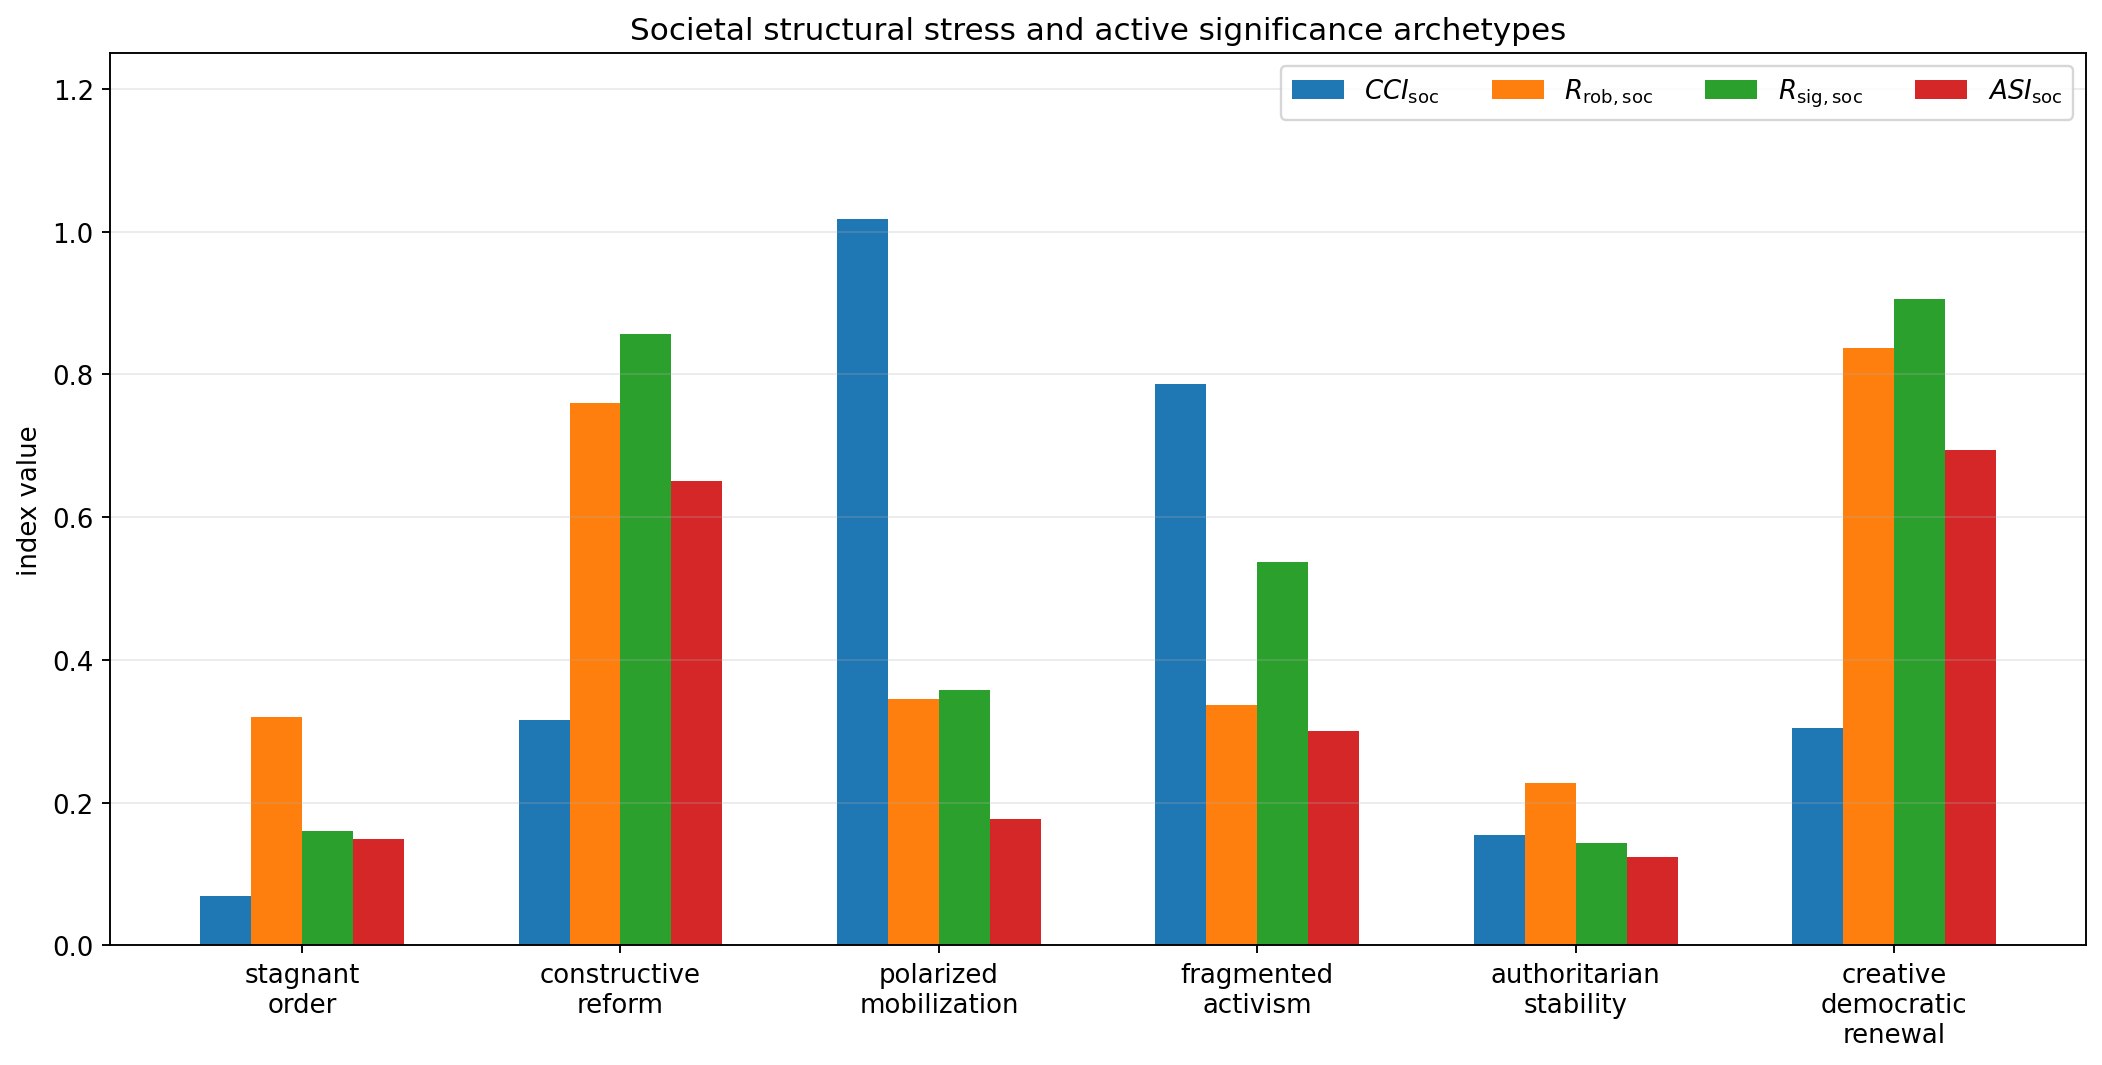
\includegraphics[width=0.96\linewidth]{fig1_societal_indices_by_archetype.png}
\caption{Synthetic archetype comparison.
Constructive reform and creative democratic renewal reach high active
significance without maximal structural stress.}
\label{fig:archetypes}
\end{figure}

\begin{figure}[H]
\centering
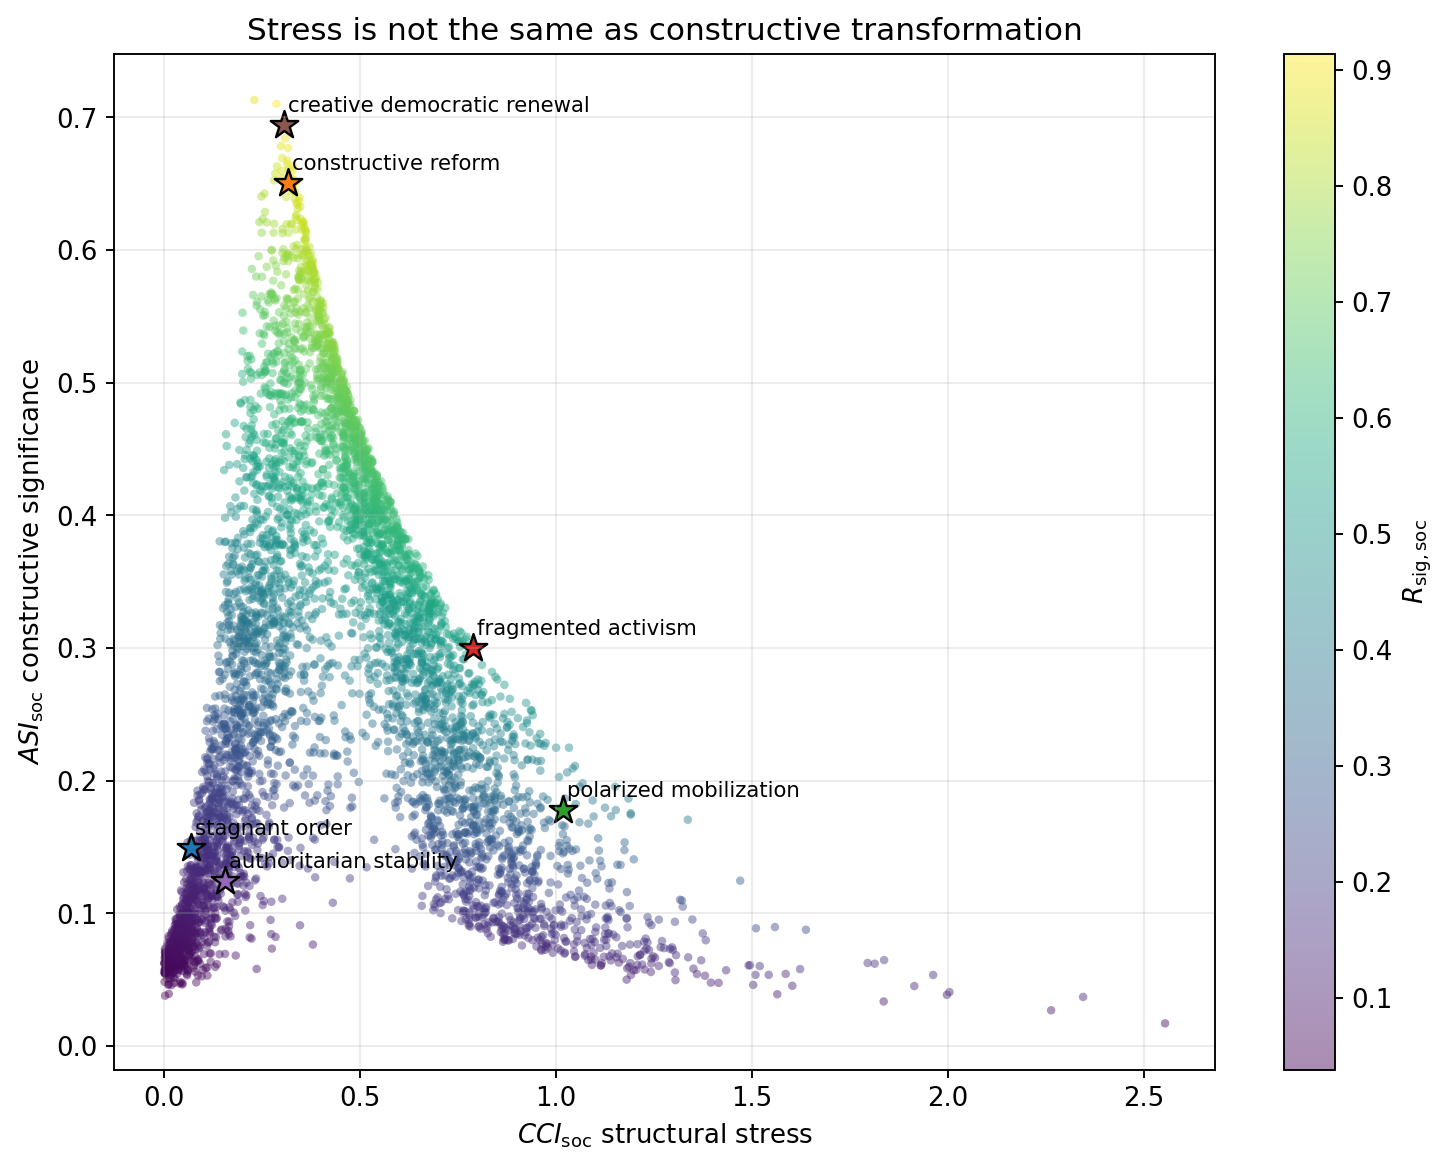
\includegraphics[width=0.82\linewidth]{fig2_stress_vs_significance_phase_space.png}
\caption{Synthetic phase-space view.
Structural stress and constructive significance are not equivalent.
High activity can be polarising, while low stress can be stagnant.}
\label{fig:phase}
\end{figure}

\begin{figure}[H]
\centering
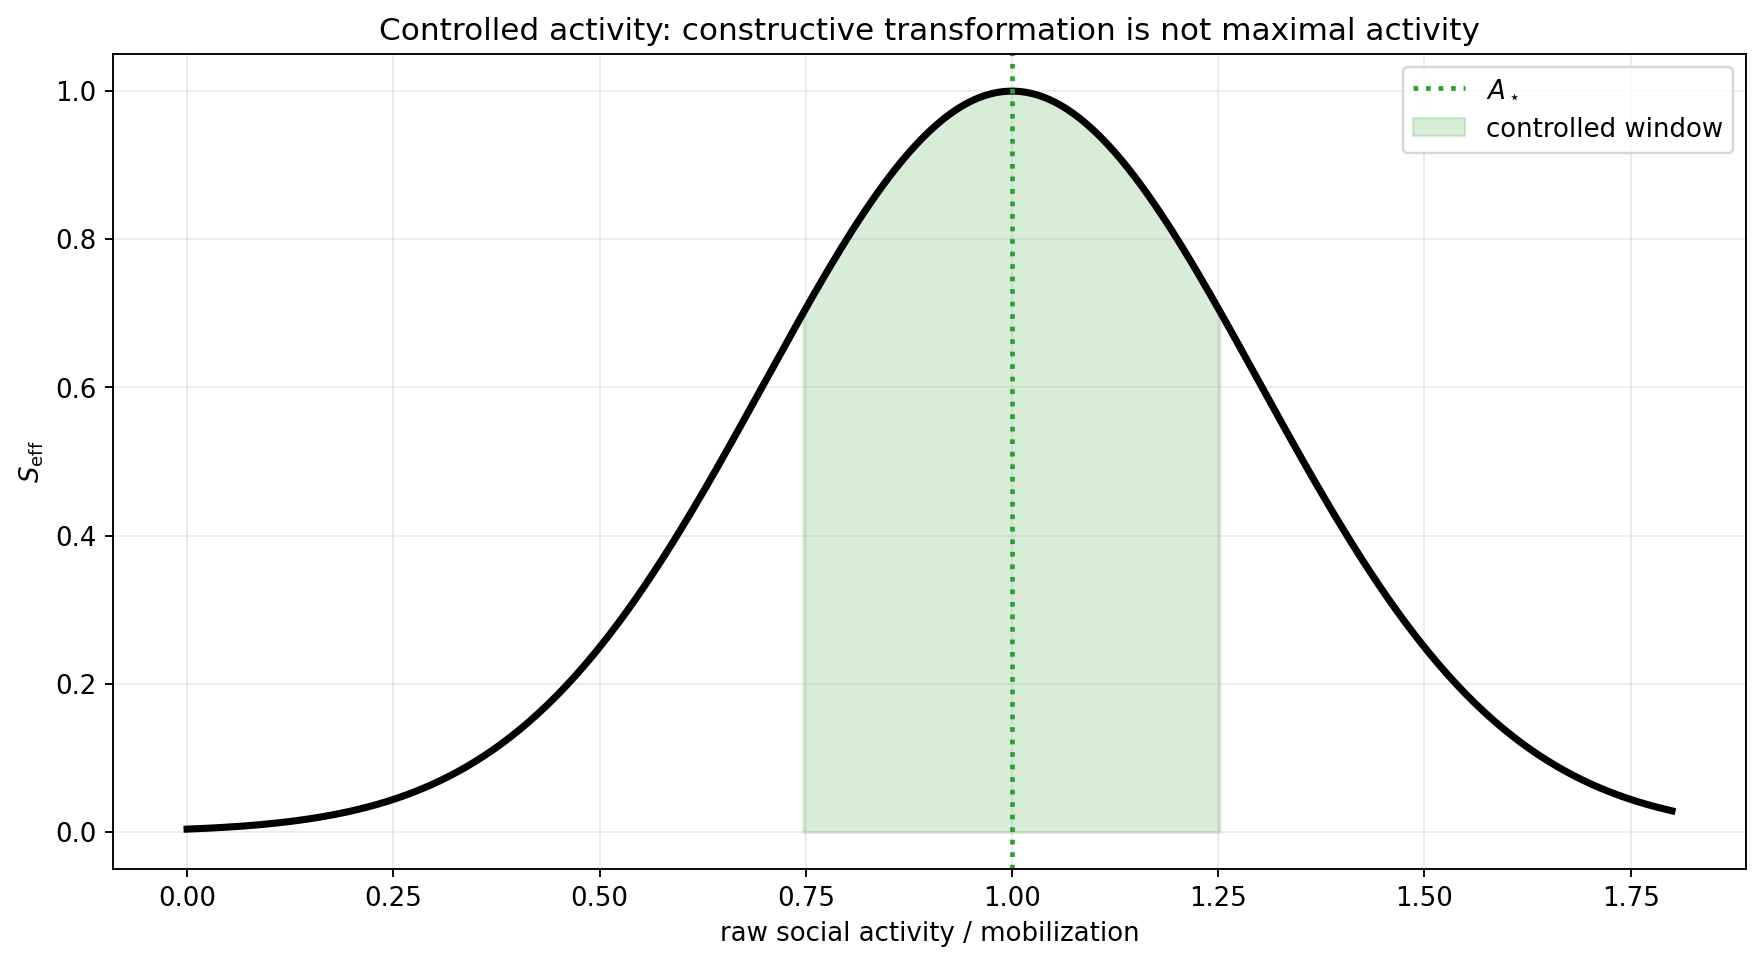
\includegraphics[width=0.86\linewidth]{fig3_controlled_activity_window.png}
\caption{Controlled activity window.
Constructive transformation is modelled as activity near an optimal window,
not as maximal raw activity.}
\label{fig:activity}
\end{figure}

In the 5000-sample synthetic ensemble, the largest regime is mixed, followed
by constrained stability and polarization-risk states:
\begin{table}[H]
\centering
\caption{Synthetic ensemble regime counts, fixed seed 44.}
\begin{tabular}{lr}
\toprule
\textbf{Regime} & \textbf{Count} \\
\midrule
mixed regime & 2876 \\
constrained stability & 784 \\
polarization risk & 672 \\
fragmentation risk & 379 \\
constructive transformation & 221 \\
stable but stagnant & 68 \\
\bottomrule
\end{tabular}
\end{table}

\begin{figure}[H]
\centering
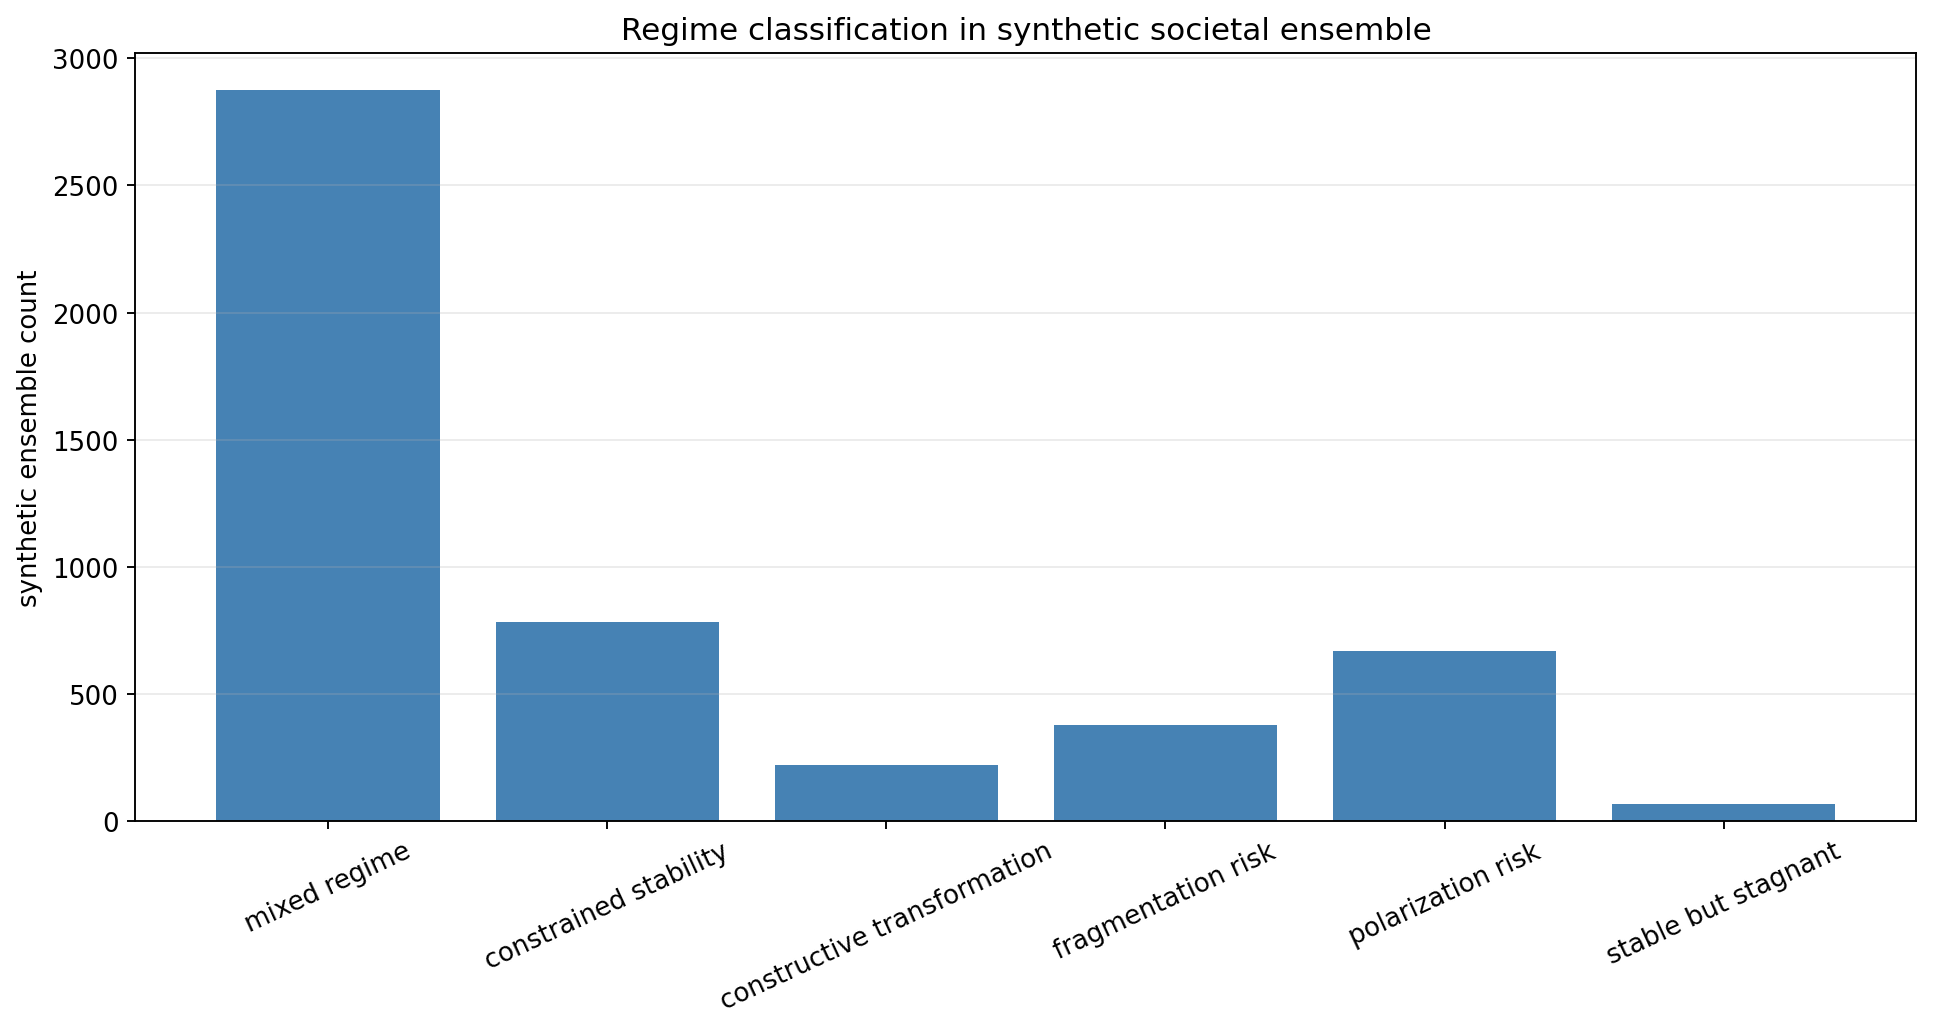
\includegraphics[width=0.90\linewidth]{fig4_synthetic_regime_counts.png}
\caption{Regime counts in the synthetic random ensemble.}
\label{fig:regimes}
\end{figure}

\section{Interpretation}

The toy model demonstrates three separations:
\begin{itemize}[leftmargin=1.5em]
\item Low stress is not sufficient for constructive transformation.
\item High activity is not sufficient for social significance.
\item Active significance requires controlled activity supported by coherence,
balance, and connectedness.
\end{itemize}

The stagnant-order archetype has low structural stress
($\CCIsoc\simeq0.069$) but also low constructive significance
($\ASIsoc\simeq0.150$).
The polarized-mobilisation archetype has the highest stress
($\CCIsoc\simeq1.018$) but low constructive significance
($\ASIsoc\simeq0.178$).
The creative-democratic-renewal archetype has high controlled activity,
high robustness, and the highest constructive significance
($\ASIsoc\simeq0.694$).

\section{Limitations}

This framework is intentionally limited:
\begin{itemize}[leftmargin=1.5em]
\item The archetypes are synthetic and do not represent real societies.
\item The support values are phenomenological.
\item The regime classifier is heuristic.
\item No causal claims are made.
\item No empirical political, cultural, demographic, or institutional data are
used.
\item The model should not be used for governance, surveillance, persuasion,
or political scoring.
\end{itemize}

\section{Reproducibility}

The experiment is stored in the repository under:
\begin{center}
\texttt{experiments/societal\_cci/}
\end{center}

Run:
\begin{verbatim}
python3 societal_cci_toy.py
\end{verbatim}

The script writes:
\begin{itemize}[leftmargin=1.5em]
\item \texttt{outputs/societal\_cci\_results.json},
\item \texttt{outputs/societal\_cci\_archetypes.csv},
\item \texttt{outputs/societal\_cci\_ensemble.csv},
\item four PNG figures used in this paper.
\end{itemize}

The public research repository is:
\begin{center}
\url{https://github.com/Chris4081/structural-selection-principle}
\end{center}

\section{Conclusion}

We introduced a synthetic Societal Critical Coherence Index as an ethical toy
extension of the MAAT/CCI framework.
The model distinguishes raw activity from controlled activity, passive
adherence from active significance, and low stress from constructive
transformation.

The main conceptual result is that social structure cannot be evaluated by
stability or activity alone.
In this toy framework, constructive transformation emerges only when activity
is held inside a coherent, balanced, and connected structural envelope.

\begin{thebibliography}{99}

\bibitem{haken1983}
H.~Haken,
\emph{Synergetics: An Introduction},
Springer, Berlin (1983).

\bibitem{luhmann1995}
N.~Luhmann,
\emph{Social Systems},
Stanford University Press, Stanford (1995).

\bibitem{ostrom1990}
E.~Ostrom,
\emph{Governing the Commons: The Evolution of Institutions for Collective
Action},
Cambridge University Press, Cambridge (1990).

\bibitem{putnam2000}
R.~D. Putnam,
\emph{Bowling Alone: The Collapse and Revival of American Community},
Simon \& Schuster, New York (2000).

\bibitem{kriegPaper44}
C.~Krieg,
``Active Structural Significance:
A Toy Extension of the MAAT v1.2.1 Robustness Closure,''
preprint (2026).

\end{thebibliography}

\end{document}
